\chapter{Design of AcCAPPCHA}
The structure and behaviour of AcCAPPCHA are similar to the ones proposed in Invisible CAPPCHA application but adding also other task to improve the efficiency. The two phases of the verification are:
\begin{itemize}
\item{Evaluation of the user activity}
\item{Comunication of the password to remote service}
\end{itemize}
In the first phase, the application exploits data from the microphone instead of using other sensors as described in AcCAPPCHA. The CAPPCHA records two audio signals: the first one created during the insertion of the password by the user and the second one created before this activity for noise evaluation. The second signal is exploited to evaluate a noise threshold usefull for the computation of amplitude peaks in the first audio.\\
During the insertion of the password, the instant of the time when each character was typed by the user is stored. Then the first verification is performed by looking if there exists a sequence of time instants of the peaks in the first signal that matches with the time instants stored manually for each character.\\
In the second phase, the username and the password of the user will be signed through ECDSA and sent by client to the authentication service if and only if the insertion was performed by a human.

\section{Time correspondence}
The correspondence between the sequence of time instants, stored looking at the software clock, and the time instants of the audio signal is performed looking for a subsequence of audio peaks. \\
First of all, the program records an audio of 1 second before asking user to insert the password. The signal will be analysed to find its maximum value, that will be used as a threshold for the identification of the peaks. In fact, the signal samples of the audio recorded during the insertion, with value higher than the last threshold, will be considered as feasible peaks.\\
These samples are then grouped in several 5 ms windows and for each of them, the application find the time instant related to the maximum value of the signal in this window. For example, given \textit{the sampling period or interval} $t_s$ and a specific window of samples: $$x = [x_t, x_{t+t_s}, ..., x_{t+\lceil \frac{10ms}{t_s}\rceil * t_s}]$$
then we compute $t'= argmax(x)$.\\
Then we declare that there is a time correspondence if given the sequence of computed time instants relative to max value of each window $t=[t_1, t_2, ..., t_n]$ if there exists a subset of it $t^{*}$ with size equal to the length of the password and that matches with a threshold with the sequence of time instants stored during the password insertion.

\section{Deep learning classification}
When pressed each key of the keyboard produces a variation of the signal, called \textit{press peak}, for a time window of about 8-10 ms\cite{keyboard_acoustic}. This signal trend can also be divided in three consecutive and distinctive areas:
\begin{itemize}
\descItem{touch peak}{peak in a window of 2-3 ms, caused by the finger touching the key}
\item{\textbf{noisy meaningless area}}
\descItem{hit peak}{peak in a window of 2-3 ms, caused by the finger and the key hitting the keyboard supporting plate.}
\end{itemize}
To obtain a prediction of each key pressed by the user, we can extract information from the touch peak, that is the most significant, and the hit peak, that increases the information related to the pression.\\
Following the idea of Asonov and Agrawal, I exploit deep learning to classify each pressed key. I use three different approaches, the first two were taken from the work of Asonov and Agrawal and the last one was based on modern sound classification techniques.\\
Respectively to the method used, the feature for each key was composed by:
\begin{itemize}
\item{FFT coefficients of the touch peak}
\item{FFT coefficients of the hit peak and the touch peak}
\item{Features obtained from the hit peak and the touch peak using a deep learning pre-trained model}
\end{itemize}
In the first two cases, the coefficients are extracted from a window of 3 ms around the peaks and then they are normalized in floating point values in range $[0, 1]$ (see Figure \ref{design:feature_example}).\\
In the third case, the touch peak and the hit peak samples were concatenated, creating a new signal on which the spectrogram is computed. From the spectrogram, I extract a feature composed by 512 values through the use of VGG16 pre-trained convolutional neural network.\\
In this way, I remove the last fully connected layers, used for classification of other task, and take the intermediate results as feature. The reason of this approach is that a pre-trained network already extracts very well features for classification of a lot of common immages and so it can extract features better than a NN created from scratch.
\begin{figure}[h]
     \centering
     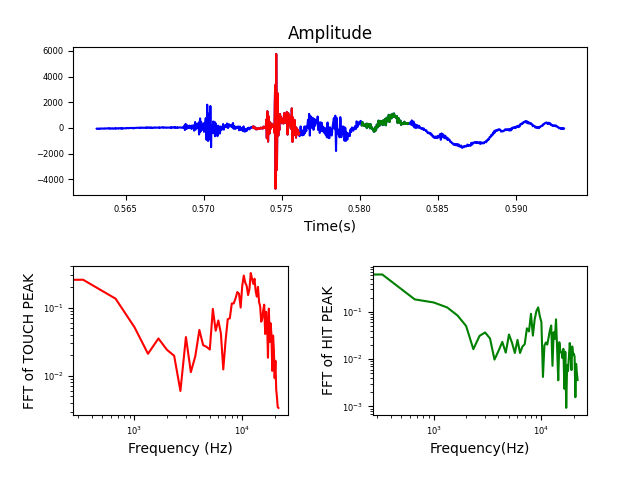
\includegraphics[width=.9\linewidth]{Images/Design/feature_example}
     \caption{\footnotesize{Example of normalized FFT computation for the touch and the hit peak.}}\label{design:feature_example}
\end{figure}\\
The audio signal taken, during the insertion of the password, is analysed and then organized in windows as specified in the previous Section, but the prediction can be done in two different ways:
\begin{itemize}
\item{on every window previously computed}
\item{on the windows that contains the time instants related to the time correspondence}
\end{itemize}
In the first approach the application uses the maximum value of each window as the touch peak and looks for the related hit peak, taking it about 10 ms after the previous peak. Then I collect the most probable keys predicted from the Neural Network for this peaks and I repeat the procedure for every window initially computed on the audio. This method is very weak because after this phase, the algorithm tries to find an ordered sequence of characters, one from each window, that corresponds with the password inserted by the user. If this exists, AcCAPPCHA declares that the user was a human, otherwise a bot. The main problem of this approach is that there is no correspondence in time between a character belonging to the final sequence and the moment in which the same character was inserted physically by the user. In fact there can be false positives caused by the prediction from peak that are not related to the absolute maximum one. In other terms, in the set of the maximuma of all the windows there can be someone that is not related to the touch peak but to a local maximum.\\
The second approach solves the previous problem because the windows, where the maxima are looked for, are obtained by the correspondence time approach. In this case, AcCAPPCHA verification becomes more accurate in theory even if in practice the deep learning technique is not very efficient.